%
% CSML Final Project Paper
%

\documentclass[11pt,a4paper]{article}
\usepackage[hyperref]{acl2019}
\usepackage{times}
\usepackage{latexsym}
\usepackage{mathtools}
\usepackage{amsmath}
\usepackage{amsfonts}
\usepackage{amssymb}
\usepackage{float}
\usepackage{graphicx}
\usepackage{caption}
\usepackage{pgfplots}
\usepackage[inline]{enumitem} % note the [inline]
\pgfplotsset{compat=newest}
\usepackage{url}

\aclfinalcopy % Uncomment this line for the final submission

\newcommand\BibTeX{B\textsc{ib}\TeX}

\title{Yahtzee: Reinforcement Learning Techniques for Stochastic Combinatorial Games}

\author{Nick Pape \\
  nap626 \\
  \texttt{nickpape@utexas.edu} \\}

\date{2025-12-01}

\begin{document}
\maketitle
\begin{abstract}
  Write your abstract here. This should be a concise summary of your work,
  including the problem you're addressing, your approach, and key results.
  Keep it to about 150-250 words.
\end{abstract}

\section{Introduction}
% 600-900 words
% 513 words so far
\subsection{Yahtzee as a Reinforcement Learning Benchmark}
While on the surface \textit{Yahtzee} appears to be a trivial dice game \cite{hasbro-2022-yahtzee-rules}, it is actually a complex stochastic optimization problem with combinatorial complexity.

Although there are methods for computing optimal play in \textit{Yahtzee} using dynamic programming, these are computationally expensive and do not scale well to multiplayer settings.
\textit{Yahtzee} offers a rich environment for testing reinforcement learning (RL) solutions due to its combination of a large but manageable state space, randomness, ease of simulation, subtle strategic considerations, and easily identifiable subproblems.
While there have been a small number of efforts to create RL agents for \textit{Yahtzee}, a comprehensive approach using self-play has yet to be published.
It remains an open question of whether deep RL methods can approach optimal performance in full-game \textit{Yahtzee}, and which architectural and training choices most affect learning efficiency and final performance.
Similarly, a robust solution for multiplayer \textit{Yahtzee} using RL methods has yet to be demonstrated.

\textit{Yahtzee} is an ideal candidate to serve as a bridge between simple toy problems such as \textit{Lunar Lander} \cite{brockman2016openai} and extremely complex games like Go \cite{silver2016alphago}.
Typical small benchmarks often offer low stochasticity and simple combinatorics whereas complex games have intractable state spaces and require massive computational resources and heavy engineering to solve.
\textit{Yahtzee} sits in a middle ground where an analytic optimum exists, but reaching it with RL methods is non-trivial.
Its blend of stochasticity and large state space makes it a challenging yet feasible benchmark for RL research.

\subsection{Objectives}

In this paper we aim to methodically study whether a deep RL agent can achieve near DP-optimal performance in full-game solitaire \textit{Yahtzee} using only self-play without any shaping rewards or expert demonstrations,
and how architectural and training choices affect learning efficiency.

Concretely, we ask: \begin{enumerate*}[label=(\roman*)]
  \item How does the trade-off between maximizing single-turn expected score and full-game performance behave?
  \item Can a shaping-free self-play agent can reach optimal performance under a fixed training budget?
  \item Which design choices (state and action encodings, variance controls, baselines, entropy, etc) most affect final performance?
  \item What failure modes exist in learned policies and how can they be addressed?
  \item Can we find a successful architecture which could be adapted to multiplayer \textit{Yahtzee}?
\end{enumerate*}

\section{Related Work}
% 600-800 words
% 742 words so far

\subsection{Policy Gradient Methods and Variance Reduction}
Policy-gradient methods are a family of algorithms which directly optimize a parameterized policy $\pi_{\theta}$ to follow an estimate of the performance gradient \cite{sutton-2000-policy-gradient}.
A simple formulation of this is the REINFORCE algorithm \cite{williams-1992-reinforce}, which uses Monte-Carlo returns $G_{t}^{MC}$ on finite, episodic tasks; however, while unbiased, it suffers from high variance.
Actor-critic methods \cite{konda-1999-actorcritic, mnih-2016-a3c} address this by learning a seperate value function, the critic $V_{\phi}$, which serves a variance reducing baseline.
A recent and popular algorithm, proximal policy optimization (PPO) \cite{schulman-2017-ppo}, utilizes a clipped objective $L^{CLIP}(\theta)$
and explicit Kulback-Leibler (KL) divergence control to dramatically reduce variance and ensure stable updates.

In long episodic games, the choice of return calculation affects sample efficiency, bias, and variance. Monte-Carlo (MC) returns $G_{t}^{MC}$ use a summation over the full series of rewards until the end of the episode.
This approach is unbiased but has high variance.
Temporal Difference returns calculate the TD-error term $\delta_t$ using a bootstrapped estimate for the value of the next state \cite{sutton-1988-temporal-differences}, which is biased but has lower variance.
n-step returns $G_{t}^{TD(n)}$ \cite{sutton-2018-reinforcement-book} interpolate between MC and single-step TD returns, allowing us to define a time horizon $n$ over which to sum rewards before bootstrapping, this lets us manually control the bias-variance tradeoff.
This is improved by the $TD(\lambda)$ algorithm \cite{sutton-2018-reinforcement-book}, which uses an exponentially weighted average of n-step returns, effectively blending multiple time horizons.
Actor-Critic and PPO can use any of these return estimation methods, including the generalized advantage estimate (GAE) \cite{schulman-2016-gae}, which is a special formulation of $TD(\lambda)$.

Aside from return estimation, there is a host of other variance reduction techniques which can be employed for policy gradient methods.
Subtracting a learned baseline from REINFORCE yields an advantage estimate that reduces variance without changing its expectation \cite{weaver2013optimal, greensmith-2004-variance-reduction}.
Normalizing advantages across a batch improves gradient conditioning and is common practice.
Entropy regularization prevents early collapse to suboptimal policies by encouraging exploration via the addition of an explicit entropy bonus term in the loss function \cite{williams-peng-1991-function-optimization}.
Gradient clipping is frequently used alongside these techniques to stop rare, but large, gradient updates from destabilizing training \cite{pascanu-2013-rnn-clipping}.
While high variance is unavoidable in deep reinforcement learning, poor performance can often be linked to numerical instability rather than inherent flaws in algorithmic design \cite{bjorck-2022-high-variance};
simple tweaks like normalizing features before activations can dramatically improve stability.

\subsection{Complex Games}
Typical board and dice games have extreme state complexity or stochasticity; reinforcement learning methods are a natural fit for these problems.
In a classic example, \citet{tesauro1995tdgammon} utilized temporal difference learning to achieve superhuman performance in \textit{Backgammon}, another game with a large state space and stochastic elements.
Tetris, which is deterministic but combinatorial, has also been studied extensively; \citet{bertsekas1996tetris} utilized approximate dynamic programming methods to learn effective policies for the game,
while \citet{gabillon2013tetris} effectively tackled the game using reinforcement learning methods.
\citet{moravcik2017deepstack} demonstrated that \textit{Texas Hold'em}, a stochastic game with hidden information, could be effectively learned.
Many other stochastic games can be learned well, so long as methods which ensure better exploration are used \cite{osband2016bootstrappeddqn}.
Lastly, RL methods can be used to reach superhuman performance on adversarial games, even despite their sparse reward structures.
For example, the game of Go, which has a notoriously intractable state space was solved using Monte-Carlo Tree Search and deep value networks \cite{silver2016alphago}.
Subsequent work showed Go could be learned without the use of expert data, purely through self-play \cite{silver2017alphagozero}.
In total, these works establish that RL methods can handle highly stochastic, combinatorial games, suggesting that \textit{Yahtzee} is a natural but underexplored candidate in this family.

\subsection{DP Methods for Yahtzee}
Solitaire \textit{Yahtzee} is a complex game with an upper bound of $~7 \times 10^{15}$ possible states in its state space.
It has a high degree of stochasticity, as dice rolls are the primary driver of state transitions.
Despite this, it has been analytically solved using dynamic programming techniques; \citet{verhoeff-1999-solitaire-yahtzee}, calculated an that the average score achieved during ideal play is $254.59$ points, which serves as the gold-standard baselline for solitaire \textit{Yahtzee}.
Later work by \citet{glenn-2006-optimal-yahtzee} optimized the DP approach via symmetries to propose a more efficient algorithm for computing the optimal policy, with a reachable state space of $~5.3 \times 10^8$ states \cite{glenn-2007-solitaire-yahtzee}.

However, adversarial \textit{Yahtzee} remains an open problem.
While \citet{pawlewicz-2011-multiplayer-yahtzee} showed that DP techniques can be expanded to 2-player adversarial \textit{Yahtzee}, they do not scale to more players due to the exponential growth of the state space.
Approximation methods must be utilized for larger player counts.

\subsection{Reinforcement Learning for Yahtzee}
Some prior attempts have been made to apply reinforcement learning to \textit{Yahtzee}.
YAMS attempted used Q-learning and SARSA to attempt to learn \textit{Yahtzee}, but was not able to surpass $~120$ points median \cite{belaich-2024-yams}.
Likewise, \citet{kang-2018-yahtzee-rl} applied hierarchical MAX-Q, achieving an average score of $129.58$ and a 67\% win-rate over a 1-turn expectimax agent baseline.
\citet{vasseur-2019-strategy-ladders} explored strategy ladders for multiplayer \textit{Yahtzee}, to understand how sensitive Deep-Q networks were to the upper-bonus threshold.
Later, \cite{yuan-2023-two-player-yahtzee} applied Deep-Q networks to the adversarial setting.

Additionally, some recent informal work has reported success using RL methods for \textit{Yahtzee}.
For example, Yahtzotron used heavy supervised pretraining and A2C to achieve an average of $~236$ points \cite{Haefner2021Yahtzotron}.
Although it is unclear if the results are repeatable, \citet{DutschkeYahtzee} reports a deep-Q agent achieving a score of $241.6 \pm 40.7$ after just 8,000 games.

No prior work systemically explores policy gradient methods with variance reduction tricks on full-game solitaire \textit{Yahtzee}, attempts transfer learning from single-turn optimization, provides a detailed ablation and failure mode analysis,
or offers an architecture that is theoretically transferrable to multiplayer settings.


\section{Problem Formulation}
% 400-600 words
\subsection{Game Description}
\subsubsection{Rules of Yahtzee}
\textit{Yahtzee} is played with five standard six-sided dice and a shared scorecard containing 13 categories.
Turns are rotated among players. A turn starts with a player rolling all five dice. They may then choose to keep
some dice, and re-roll the remaining ones. This process can be repeated up to two more times, for a total of three rolls.
After the final roll, the player must select one of the 13 scoring categories to apply to their current dice.
Each category has specific scoring rules, and each can only be used once per game.

\subsubsection{Mathematical Representation of Yahtzee}
\label{sec:yahtzee-definitions}
The space of all possible dice configurations is:
$$\mathcal{D} \in \{1, 2, 3, 4, 5, 6\}^5$$
and the current state of the dice is represented as:
$$\mathbf{d} \in \mathcal{D}$$

In addition, we can represent the score card as a vector of length 13, where each element corresponds to a scoring category:

$$\mathbf{c} = (c_1, c_2, \ldots, c_{13}) \text{ where } c_i \in \mathcal{D}_i \cup \{\varnothing\}$$

and $\varnothing$ indicates an unused category.

Let us also define a dice face counting function which we can use to simplify score calculations:
\begin{align*}
  n_v(\mathbf{d})        & = \sum_{i=1}^{5} \mathbb{I}(d_i = v),
  \quad v \in \{1,\dots,6\}                                                  \\
  \mathbf{n}(\mathbf{d}) & = \big(n_1(\mathbf{d}),\dots,n_6(\mathbf{d})\big)
\end{align*}

Let the potential score for each category be defined as follows (where detailed scoring rules can be found in Appendix~\ref{app:scoring}):
\begin{align*}
  \mathbf{f}(\mathbf{d}) & =
  \bigl(f_1(\mathbf{d}), f_2(\mathbf{d}), \ldots, f_{13}(\mathbf{d})\bigr)
\end{align*}

The current turn number can be represented as:
$$t \in \{1, 2, \ldots, 13\}, \quad t = \sum_{i=1}^{13} \mathbb{I}(c_i \neq \varnothing)$$

A single turn is composed of an initial dice roll, two optional re-rolls, and a final scoring decision.
Let $r = 0$, with $r \in \{0,1,2\}$ which is the number of rolls taken so far.
Prior to the first roll, the dice are randomized:
$$
  \mathbf{d}_{r=0} \sim U(\mathcal{D})
$$

The player must decide which dice to keep and which to re-roll. Let the player define a keep vector:
$$\mathbf{k} \in \{0,1\}^5$$
where $\mathbf{k}_i = 1$ indicates that die $i$ is kept, otherwise it is re-rolled.

We can then define the transition of the dice state after a re-roll as:
\begin{align*}
  \mathbf{d}' & \sim U(\mathcal{D}),                          \\[2pt]
  \mathbf{d}_{r+1}
              & = (\mathbf{1} - \mathbf{k}) \odot \mathbf{d}'
  + \mathbf{k} \odot \mathbf{d}
\end{align*}


When $r=2$, the player must choose a scoring category to apply their current dice to. Define a scoring choice mask as a one-hot vector:
$$\mathbf{s} \in \{0,1\}^{13}, \quad \|\mathbf{s}\|_1 = 1$$

For the purposes of calculating the final (or current) score, any field that has not been scored yet can be counted as zero.
We can define a mask vector for this:

\begin{align*}
   & \mathbf{u}(\mathbf{c}) \in \{0,1\}^{13}                                                                     \\
   & \mathbf{u}(\mathbf{c})_i = \mathbb{I}\bigl(c_i \neq \varnothing\bigr), \quad \forall i = \{ 1, \ldots 13 \}
\end{align*}


If a player achieves a total score of 63 or more in the upper section (categories 1-6), they receive a bonus of 35 points:
$$
  B(\mathbf{c}) = \begin{cases}
    0,  & 63 \leq \sum_{i=1}^{6} \mathbf{u}(\mathbf{c})_i \cdot \mathbf{c}_i \\
    35, & \text{otherwise}
  \end{cases}
$$

The player's score can thus be calculated as:
$$\mathrm{score}(\mathbf{c}) = B(\mathbf{c}) + \big\langle \mathbf{u}(\mathbf{c}), \mathbf{c} \big\rangle$$

\subsection{MDP Formulation}
We model \textit{Yahtzee} as a Markov Decision Process $(\mathcal S,\mathcal A,P,R,\gamma)$ \citep{Puterman1994MDP}.

A state is represented as $\mathbf{s} = (\mathbf{d},\mathbf{c},r, t)$, where $\mathbf{d}$ is the current
dice configuration, $\mathbf{c}$ the scorecard, and $r$ the roll index, and $t$ the current turn index
(see Section~\ref{sec:yahtzee-definitions}).

For simplicity, we define the action $\mathbf{a} = (\mathbf{k}, \mathbf{s})$, where $\mathbf{k}$ is the keep vector and $s$ is the score category choice.
We can define the action as a parameterization of the policy: $\pi_{\theta}(\mathbf{a}|\mathbf{s}) = \pi_{\theta}(\phi(\mathbf{s}))$,
where $\phi(\mathbf{s})$ is a feature representation of the state $\mathbf{s}$.

The transition function $P$ is is specified in Appendix~\ref{app:transition-function}. Note that when $r < 2$, the $\mathbf{k}$ is used by $P$, otherwise $\mathbf{s}$ is used.

The reward is the change in total score between steps $R_t = \mathrm{score}(c_{t+1}) - \mathrm{score}(c_t)$,
and since we desire to maximize total score at the end of the game, we set $\gamma = 1$.


\subsection{Single-Turn Optimization Task}
In the single-turn optimization task, the agent is trained to maximize the expected score over a single turn.
This task has 3 steps total; after being initialized with a random dice roll, the agent chooses which
dice to keep and which to re-roll twice, and then selects a scoring category. A single reward is given at the end of the turn.

This is a useful subproblem to study, as it isolates the decision-making process in a single turn,
allowing us to analyze the network architecture and training regime in a low-variance setting.

\subsection{Full-Game Optimization Task}
In the full-game optimization task, 13-turn episodes are played to completion.
The objective again is to maximize the total score at the end of the game.
This task is more challenging due to the longer horizon, increased variance, and the requirement for
the network to learn explicit long-term strategies, such as planning for the upper bonus.

\section{Methodology}
1400-1700 words
\subsection{State Representation \& Input Features}
The design of $\mathbf{\phi}(\mathbf{s}) \rightarrow \mathbf{x}$ is one of the most critical components to the performance of a model \cite{sutton-2018-reinforcement-book}.

As such, several different representations were tested to evaluate their impact on learning efficiency and final performance.

\subsubsection{Dice Representation}
The dice representation can be encoded in several ways, depending on if we want to preserve permutation invariance or not.
Preserving ordering information (and implicitly, ranking) gives the model the benefit of being able to directly output actions corresponding to dice indices,
however, it comes at the cost of implicitly biasing the model to specific dice orderings; in other words, towards a local optima of keeping the highest ranking dice.
However, eliminating ordering information requires the model to either waste capacity learning permutation invariance or be inherently supportive of invariance (e.g. with self-attention).
It also requires a different action representation, since actions can no longer correspond to specific dice indices. We attempted 5 different dice representations:

\begin{itemize}
  \item \textbf{One-hot encoding of ordered dice:} Each die is represented as a one-hot vector of length 6, and the 5 dice are concatenated in order.
  \item \textbf{Bin representation:} Here we pass through the dice face count vector $\mathbf{n}(\mathbf{d})$.
  \item \textbf{Combined representation:} Both ordered one-hot and bin representations are concatenated.
  \item \textbf{Learnable encoding of dice:} Each die is represented as a learnable embedding vector of length $d$, and self-attention is applied.
  \item \textbf{Learnable encoding of dice with positional encodings:} Similar to above, but with sinusoidal positional encodings added to each die embedding.
\end{itemize}

$$\phi_{\mathrm{dice}}(\mathbf{d}) = \text{(varies by representation)}$$

\subsubsection{Scorecard Representation}
There are two important pieces of information $\mathbf{\phi}$ must encode about the scorecard: whether a category is open or closed,
and some form of progress towards the upper bonus.
$$\phi_{\mathrm{cat}}(\mathbf{c}) = \mathbf{u}(\mathbf{c})$$

We experimented with several ways of encoding the bonus progress, but settled on a simple normalized, clamped sum of the upper section scores:
$$\phi_{\mathrm{bonus}}(\mathbf{c}) = \min\biggl(\frac{1}{63} \sum_{i=1}^{6} c_{i}, 1\biggr)$$

\subsubsection{Computed Features}
There are some key features that can be computed from the raw state, providing these can allow the model to focus on higher-level patterns.

\begin{align*}
  \phi_{\mathrm{progress}}(t)       & = \frac{t}{12}                                                                        \\[4pt]
  \phi_{\mathrm{rolls}}(r)          & \in \{0,1\}^3, \quad \|\phi_{\mathrm{rolls}}(r)\|_1 = 1                               \\[4pt]
  \phi_{\mathrm{joker}}(\mathbf{c}) & \in \{0,1\}, \quad \text{(Joker rule active)}                                         \\[4pt]
  \phi_{\mathrm{potential}}(\mathbf{d}, \mathbf{c})
                                    & = \bigl(\mathbf{u}(\mathbf{c}) \odot \mathbf{f}(\mathbf{d})\bigr) \oslash \mathbf{m},
\end{align*}
where $m_k = \max_{\mathbf{d}'} f_k(\mathbf{d}')$ is the maximum possible score for category $k$.


\subsection{Action Representation}
\subsubsection{Rolling Action}
We experiment with two different rolling action representations.
The first is a Bernoulli representation, where each die has an individual binary decision to be re-rolled or held.
The second is a categorical representation, where each of the 32 possible combination of dice to keep is represented as a unique action.

\[
  a_{\mathrm{roll}} \sim
  \begin{cases}
    \mathrm{Bernoulli}\!\left(\sigma\!\left(f_\theta(\phi(x))\right)\right) \\
    \mathrm{Categorical}\!\left(\mathrm{softmax}\!\left(f_\theta(\phi(x))\right)\right)
  \end{cases}
\]

\subsubsection{Scoring Action}
The scoring action is always a categorical distribution over the 13 scoring categories.
\[
  a_{\mathrm{score}} \sim \mathrm{Categorical}\!\left(\mathrm{softmax}\!\left(f_\theta(\phi(x))\right)\right)
\]

\subsection{Neural Network Architecture}
The neural network uses a unique architecture designed to handle the specific challenges of \textit{Yahtzee}.
The architecture consists of a trunk, followed by heads for the policy and value functions.

\subsubsection{Trunk}
The trunk of the network is a standard feedforward architecture with 2-3 fully connected hidden layers.
The width of each layer is 386-512 neurons, found through empirical hyperparameter tuning,
but aligning our model capacity with theoretical maximums \cite{horne-1994-bounds-rnn-fsm} and minimums \cite{hanin-2017-bounded-width-relu}.
We utilize layer normalization for improved training stability \cite{ba-2016-layernorm, bjorck-2022-high-variance}
and Swish activations \cite{ramachandran-2017-swish} to introduce stable non-linearities.

\subsubsection{Policy and Value Heads}
We utilize two distinct heads for the rolling and scoring actions, allowing the model to specialize in
each task \cite{tavakoli2018actionbranching, hausknecht2016parameterized}.

\subsubsection{Weight Initialization}
<KAIMING OR XAVIER?>

\subsubsection{Optimization \& Schedules}
We utilize the Adam optimizer \cite{kingma2014adam} with maximum learning rate between $1\times 10^{-4}$ and $5\times 10^{-4}$.
To improve training stability, we utilize a warmup schedule over the first 5\% of training \cite{kalra-2024-warmup},
plateau for 70\% of training, and then linearly decay over the final 25\% of training steps \cite{defazio2023optimal, lyle2024normalization}.

\subsubsection{Training Metrics}
To better understand training dynamics, we log several metrics during training.
To monitor the quality of the value network, we monitor explained variance \cite{schulman2016nutsbolts, schulman-2016-gae}.
To monitor for policy collapse, we track the policy entropy and KL divergence between policy updates \cite{schulman2016nutsbolts,schulman-2017-ppo},
mask diversity \cite{Hubara2021MaskDiversity},
and the top-k action frequency \cite{sun-etal-2025-curiosity}.
To monitor for learning stability, we track gradient norms and clip rate \cite{pascanu-2013-rnn-clipping, Engstrom2020ImplementationMatters}.
To ensure advantages are well-conditioned, we track advantage mean and standard deviation \cite{Achiam2018SpinningUp}.
We also monitor standard training metrics such as average reward and loss values.

\subsection{Reinforcement Learning Algorithms}
\subsubsection{REINFORCE}
<Talk about REINFORCE loss function, how it is used with baseline, single vs full game, etc.>
\subsubsection{TD}
<Talk about TD(n) and TD(lambda), how they are used with actor-critic, application to full game, etc.>
\subsubsection{PPO}
<Talk about PPO loss function, clipping, KL control, application to full game, etc.>

\subsection{Training Regimes}
<Talk about single-turn vs full-game training, transfer learning, etc.>
\subsubsection{Evaluation Protocol}
<Talk about how many eval games, deterministic vs stochastic eval, etc.>

\section{Results}

\subsection{Generalization of Single-Turn Agent to Full Game}
<200-400 words>
<Talk about the single-turn agent's performance when directly applied to full-game Yahtzee without further training.>
<Tradeoff with full-game performance, etc.>

\subsection{Single-Turn Results}
<600-700 words>
\subsubsection{Baseline Model Performance}

\begin{table}[H]
  \centering
  \caption{Category statistics for the optimal strategy}
  \label{tab:category-stats}
  \begin{tabular}{lcc}
    \hline
    \multicolumn{1}{c}{\emph{Category}} & $\bar{s}(c)$ & $\sigma^{2}(c)$ \\
    \hline
    Ones                                & <X>          & <Y>             \\
    Twos                                & <X>          & <Y>             \\
    Threes                              & <X>          & <Y>             \\
    Fours                               & <X>          & <Y>             \\
    Fives                               & <X>          & <Y>             \\
    Sixes                               & <X>          & <Y>             \\
    Three of a Kind                     & <X>          & <Y>             \\
    Four of a Kind                      & <X>          & <Y>             \\
    Full House                          & <X>          & <Y>             \\
    Small Straight                      & <X>          & <Y>             \\
    Large Straight                      & <X>          & <Y>             \\
    Chance                              & <X>          & <Y>             \\
    Yahtzee                             & <X>          & <Y>             \\
    Upper Bonus                         & <X>          & <Y>             \\
    Yahtzee Bonus                       & <X>          & <Y>             \\
    \hline
  \end{tabular}
\end{table}


\begin{figure}[t]
  \centering
  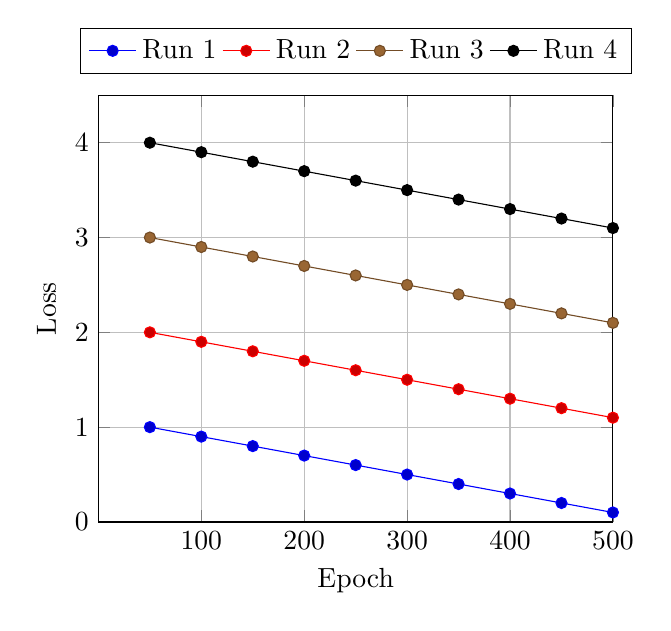
\begin{tikzpicture}
    \begin{axis}[
        height=7cm,
        xlabel={Epoch},
        ylabel={Loss},
        xmin=0, xmax=500,
        ymin=0, ymax=4.5,
        xtick={100,200,300,400,500},
        grid=both,
        legend style={at={(0.5,1.05)},anchor=south,legend columns=4},
        mark options={solid},
      ]

      % --- Run 1 (placeholder data around 1) ---
      \addplot+[mark=*] coordinates {
          ( 50,1.0) (100,0.9) (150,0.8) (200,0.7) (250,0.6)
          (300,0.5) (350,0.4) (400,0.3) (450,0.2) (500,0.1)
        };

      % --- Run 2 (placeholder data around 2) ---
      \addplot+[mark=*] coordinates {
          ( 50,2.0) (100,1.9) (150,1.8) (200,1.7) (250,1.6)
          (300,1.5) (350,1.4) (400,1.3) (450,1.2) (500,1.1)
        };

      % --- Run 3 (placeholder data around 3) ---
      \addplot+[mark=*] coordinates {
          ( 50,3.0) (100,2.9) (150,2.8) (200,2.7) (250,2.6)
          (300,2.5) (350,2.4) (400,2.3) (450,2.2) (500,2.1)
        };

      % --- Run 4 (placeholder data around 4) ---
      \addplot+[mark=*] coordinates {
          ( 50,4.0) (100,3.9) (150,3.8) (200,3.7) (250,3.6)
          (300,3.5) (350,3.4) (400,3.3) (450,3.2) (500,3.1)
        };

      \legend{Run 1,Run 2,Run 3,Run 4}

    \end{axis}
  \end{tikzpicture}
  \caption{Training loss over epochs (placeholder data).}
  \label{fig:loss-vs-epoch}
\end{figure}

<train entropy graph>

<train top k freq graph>

<train policy KL graph>

<table of per category scores and stddev>

\subsubsection{Representational Ablations}
<Show how adding some representations pushes performance up or down.>
<Graph average score vs representation choice>

\subsubsection{Architectural Ablations}
<Show how changing architecture (layer norm, activation fn, width, depth) affects performance.>
<Graph average score vs architecture choice>

\subsubsection{Summary}
<Talk about the biggest levers>

\subsection{Full-Game Results}
<600-700 words>
\subsubsection{REINFORCE}
<Talk about reusing the single-turn config and how it doesn't perform well>
<Talk about tuning it for full-game and how that helps>
<Graph showing single turn vs full game REINFORCE performance>

\subsubsection{TD($\lambda$)}
<Talk about how it performs better than REINFORCE>

\subsubsection{PPO}
<Talk about how it performs best>

\subsubsection{Transfer Learning}
<Show results for transfer learning directly>
<Show results for transfer learning with LoRA>

\subsubsection{Summary}
<Summarize full-game results and key findings>
\begin{figure}[H]
  \centering
  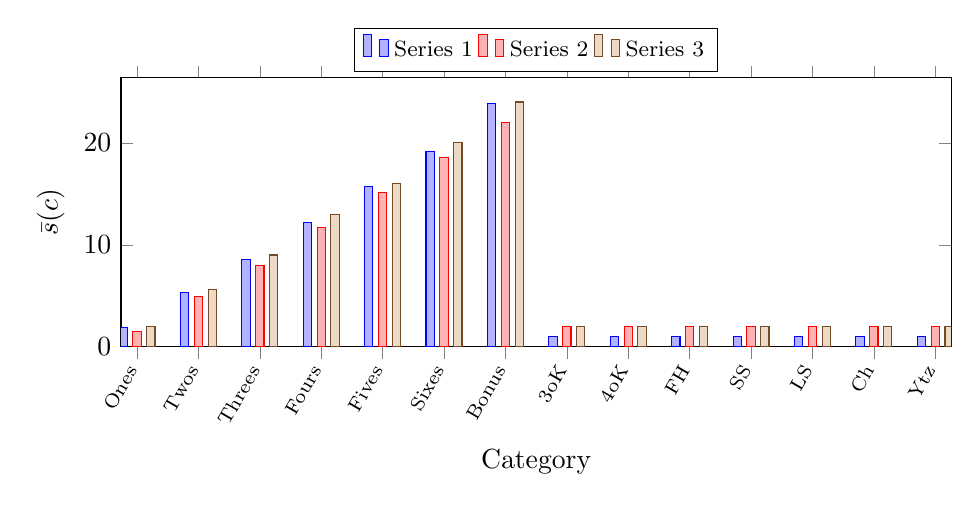
\begin{tikzpicture}
    \begin{axis}[
        ybar,
        width=\columnwidth,      % fit to single column
        height=5cm,              % a bit shorter
        bar width=3pt,
        symbolic x coords={Ones,Twos,Threes,Fours,Fives,Sixes,Bonus,3oK,4oK,FH,SS,LS,Ch,Ytz},
        xtick=data,
        xticklabel style={
            rotate=60,
            anchor=east,
            font=\scriptsize       % smaller labels
          },
        ylabel={$\bar{s}(c)$},
        xlabel={Category},
        ymin=0,
        legend style={
            at={(0.5,1.02)},
            anchor=south,
            legend columns=3,
            font=\footnotesize
          },
        enlarge x limits=0.02,   % less side padding
      ]

      % ---- Series 1 ----
      \addplot coordinates {
          (Ones,   1.88)
          (Twos,   5.28)
          (Threes, 8.57)
          (Fours,  12.16)
          (Fives,  15.69)
          (Sixes,  19.19)
          (Bonus,  23.84)
          (3oK,    1)
          (4oK,    1)
          (FH,     1)
          (SS,     1)
          (LS,     1)
          (Ch,     1)
          (Ytz,    1)
        };

      % ---- Series 2 ----
      \addplot coordinates {
          (Ones,   1.50)
          (Twos,   4.90)
          (Threes, 8.00)
          (Fours,  11.70)
          (Fives,  15.10)
          (Sixes,  18.60)
          (Bonus,  22.00)
          (3oK,    2)
          (4oK,    2)
          (FH,     2)
          (SS,     2)
          (LS,     2)
          (Ch,     2)
          (Ytz,    2)
        };

      % ---- Series 3 ----
      \addplot coordinates {
          (Ones,   2.00)
          (Twos,   5.60)
          (Threes, 9.00)
          (Fours,  13.00)
          (Fives,  16.00)
          (Sixes,  20.00)
          (Bonus,  24.00)
          (3oK,    2)
          (4oK,    2)
          (FH,     2)
          (SS,     2)
          (LS,     2)
          (Ch,     2)
          (Ytz,    2)
        };

      \legend{Series 1,Series 2,Series 3}

    \end{axis}
  \end{tikzpicture}
  \caption{Average score $\bar{s}(c)$ per category for three strategies.}
  \label{fig:yahtzee-bar}
\end{figure}


\subsection{Policy Analysis}
<300-500 words>
\subsubsection{Category Usage Distribution}
<Bar chart showing average score per category for different agents>

<table comparison against DP optimal solutions>

\subsubsection{Score Breakdown}
<Notes on how different agents achieve their scores differently>

\subsubsection{Strategy Comparison}
<Compare strategies learned by different agents>

\subsubsection{Failure Modes}
<Analyze common failure modes observed in learned policies>
<Analyze failures during training such as policy collapse>

\section{Discussion}
<400-600 words>
<Discuss implications of results, limitations, and potential improvements.>

\section{Conclusion and Future Work}
<200-300 words>
<Summarize key findings and suggest directions for future research.>

\bibliography{1_introduction,2_related_work,3_methods,4_single_turn_results,5_full_game_experiments,6_discussion,7_appendix}
\bibliographystyle{acl_natbib}

\appendix

\section{AI Usage}

This paper utilized artificial intelligence tools in the following ways:

\begin{itemize}
  \item \textbf{GitHub Copilot (Claude Sonnet 4.5)} was used for typesetting assistance with LaTeX/KaTeX and for autocomplete suggestions during coding.
  \item \textbf{ChatGPT (GPT-5)} was used for brainstorming ideas for reinforcement learning applications in games, guidance in hyperparameter tuning, helping to outline the structure of the paper, and suggesting relevant related work.
\end{itemize}

All other content, including research methodology, analysis, results interpretation, and conclusions, represents original work by the author. The AI tools were used only for initial ideation and to assist research, not for generating substantive content or analysis.

\section{Yahtzee Scoring Rules}
\label{app:scoring}
Next we define the indicator functions for each of the scoring categories:

\begin{align*}
  \mathbb{I}_{3\mathrm{k}}(\mathbf{d})
   & = \mathbb{I}\bigl\{ \max_{v} n_v(\mathbf{d}) \ge 3 \bigr\} \\[4pt]
  \mathbb{I}_{4\mathrm{k}}(\mathbf{d})
   & = \mathbb{I}\bigl\{ \max_{v} n_v(\mathbf{d}) \ge 4 \bigr\} \\[6pt]
  \mathbb{I}_{\mathrm{full}}(\mathbf{d})
   & = \mathbb{I}\Bigl\{
  \exists i, j \in \{1, \mathellipsis, 6 \} \ \text{with} \ n_i(\mathbf{d}) = 3 \land n_j(\mathbf{d}) = 2
  \Bigr\}                                                       \\[6pt]
  \mathbb{I}_{\mathrm{ss}}(\mathbf{d})
   & = \mathbb{I}\Bigl\{
  \exists k \in \{1,2,3\} \ \text{with}\
  \sum_{v=k}^{k+3} \mathbb{I}\{n_v(\mathbf{d}) > 0\} = 4
  \Bigr\}                                                       \\[6pt]
  \mathbb{I}_{\mathrm{ls}}(\mathbf{d})
   & = \mathbb{I}\Bigl\{
  \exists k \in \{1,2\} \ \text{with}\
  \sum_{v=k}^{k+4} \mathbb{I}\{n_v(\mathbf{d}) > 0\} = 5
  \Bigr\}                                                       \\[6pt]
  \mathbb{I}_{\mathrm{yahtzee}}(\mathbf{d})
   & = \mathbb{I}\bigl\{\max_v n_v(\mathbf{d}) = 5\bigr\}
\end{align*}

The potential score for each category can then be defined as:
\begin{align*}
  f_j(\mathbf{d})        & = j \cdot n_j(\mathbf{d}), \qquad j \in \{1,\dots,6\}                   \\[4pt]
  f_7(\mathbf{d})        & = \mathbf{1}^\top \mathbf{d} \cdot \mathbb{I}_{3\mathrm{k}}(\mathbf{d}) \\[4pt]
  f_8(\mathbf{d})        & = \mathbf{1}^\top \mathbf{d} \cdot \mathbb{I}_{4\mathrm{k}}(\mathbf{d}) \\[4pt]
  f_9(\mathbf{d})        & = 25 \cdot \mathbb{I}_{\mathrm{full}}(\mathbf{d})                       \\[4pt]
  f_{10}(\mathbf{d})     & = 30 \cdot \mathbb{I}_{\mathrm{ss}}(\mathbf{d})                         \\[4pt]
  f_{11}(\mathbf{d})     & = 40 \cdot \mathbb{I}_{\mathrm{ls}}(\mathbf{d})                         \\[4pt]
  f_{12}(\mathbf{d})     & = 50 \cdot \mathbb{I}_{\mathrm{yahtzee}}(\mathbf{d})                    \\[4pt]
  f_{13}(\mathbf{d})     & = \mathbf{1}^\top \cdot \mathbf{d}                                      \\[4pt]
  \mathbf{f}(\mathbf{d}) & =
  \bigl(f_1(\mathbf{d}), f_2(\mathbf{d}), \ldots, f_{13}(\mathbf{d})\bigr)
\end{align*}

\section{State Transition Function}
\label{app:transition-function}

$P$ can be defined by the following generative process.

\begin{itemize}
  \item If $r < 2$ and $a = k$, for each die $i$:
        \begin{itemize}
          \item if $k_i = 1$, keep $d'_i = d_i$;
          \item else sample $d'_i \sim \mathrm{Unif}\{1,\dots,6\}$ independently.
        \end{itemize}
        Set $c' = c,\ r' = r+1,\ t' = t$.
  \item If $r = 2$ and $a = i$, set $d' = d$, update $c' = \mathrm{score}(c,d,i)$,
        set $r' = 0,\ t' = t+1$.
\end{itemize}


\end{document}
